Med udgangspunkt i domænemodellen udviklet i arkitekturfasen er der udviklet applikationsmodeller for hver computer i systemet. Dette giver overblik over de funktionaliteter som skal implementeres på de forskellige platforme.

Applikationsmodellen består af at beskrive hvordan information fordeles i hvert UC. Dette opnåes med tre diagram typer. Sekvensdiagrammer som viser hvordan information bevæger sig sekventielt igennem systemets klasser, et klassediagram som sammenfatter de metoder og relationer som er fundet i sekvensdiagrammet og et tilstandsmaskinediagram som viser et systems forskellige tilstande. Det sidste er udeladt da det ikke er aktuelt for det opbyggede system.

\subsection{Applicationsmodel for PC (JC)}

Ud fra domænemodellen og de forskellige Use cases er der oprettet sekvens diagrammer for hver use case (UC4 og UC7 undtaget, UC4 fordi den er utrolig simpel og UC7 fordi den referere til UC8) Sekvensdiagrammet for UC2 Aktiver kan ses på nedenstående billede. Resten af sekvensdiagrammerne kan ses i rapport dokumentationen

\begin{figure}[htbp] \centering
{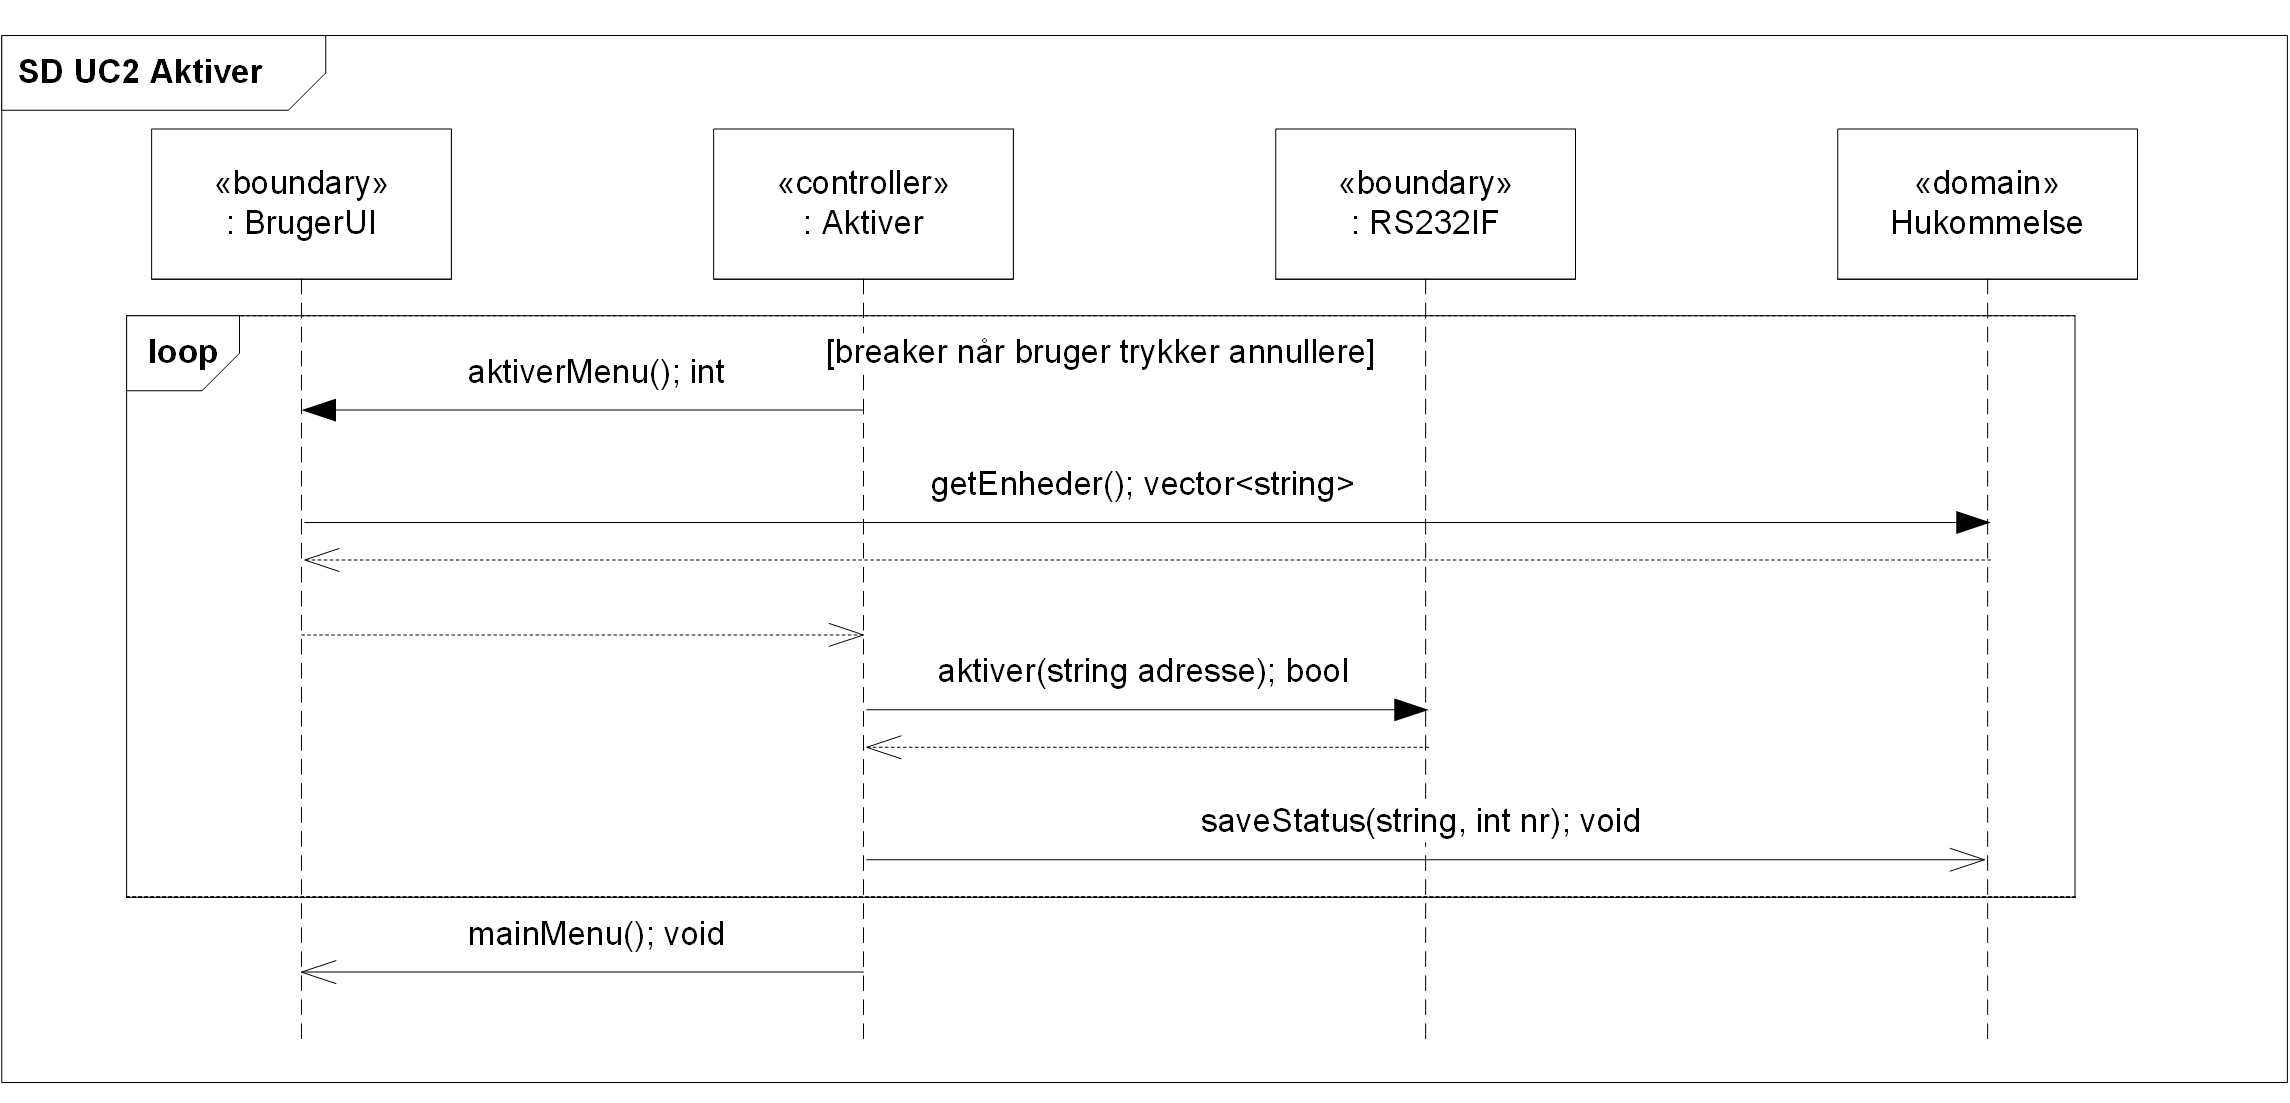
\includegraphics[width=\textwidth]{billeder/uml/PC_UC2}}
\caption{Sekvensdiagram UC2}
\label{lab:Sekvensdiagram UC2}
\end{figure}

Efter at alle sekvens diagrammerne er lavet har vi alle vores conceptuelle klasser med metoder som vi nu kan overføre til et klasse diagram som ses nedenfor

\clearpage
\begin{figure}[htbp] \centering
{\includegraphics[width=\textwidth]{billeder/uml/PC_class}}
\caption{PC klasse diagram}
\label{lab: PC klasse diagram}
\end{figure}

Når man så har lavet sit conceptuelle klassediagram kan man arbejde videre med det for at få et statisk klassediagram og klassebeskrivelser hvorefter man kan begynde sit design.

\subsection{CSS hovedenhed (BS)}

\subsection{Applikationsmodel for X10 udtag (BS)}
Først er der lavet en detaljeret domænemodel for X10 udtaget. Denne er vist i figur \ref{fig:X10_udtag_domaenemodel}. Denne laves ved at gennemgå UC beskrivelserne og finde de ting som har indflydelse på netop denne del af systemet.

\begin{figure}[!htb]
     \centering
     { 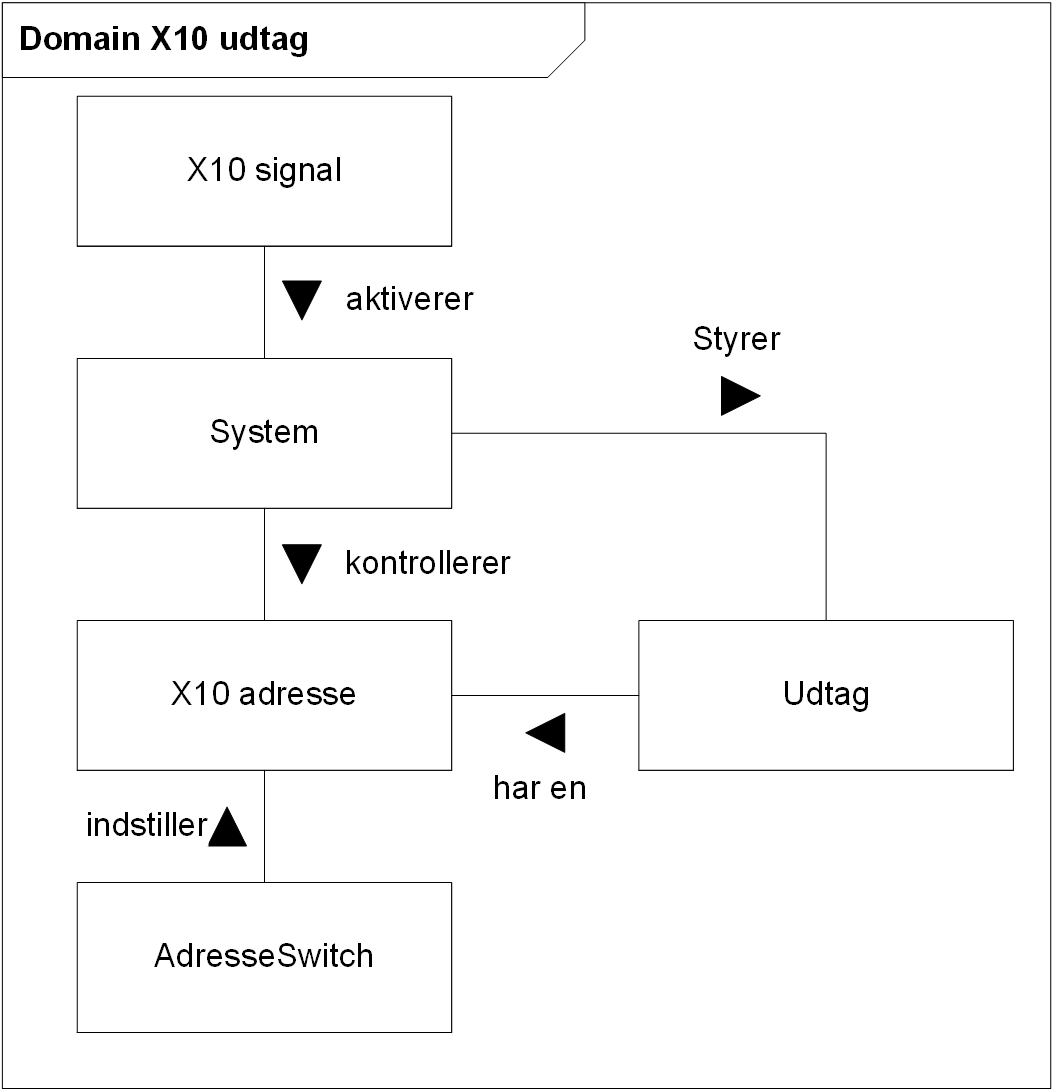
\includegraphics[width=0.9\textwidth]{Billeder/UML/X10_modtager_Domain}}
     \caption{Domænemodel for X10 udtag}
     \label{fig:X10_udtag_domaenemodel}
\end{figure}

Med dette udgangspunkt laves der sekvensdiagrammer for hvert UC. Disse er vist i figur \ref{fig:X10_udtag_sd}. De viser hvordan metodekald i mellem de konceptuelle klasser og giver et overblik over den basale funktionalitet.

\begin{figure}[!htb]
     \centering
     { 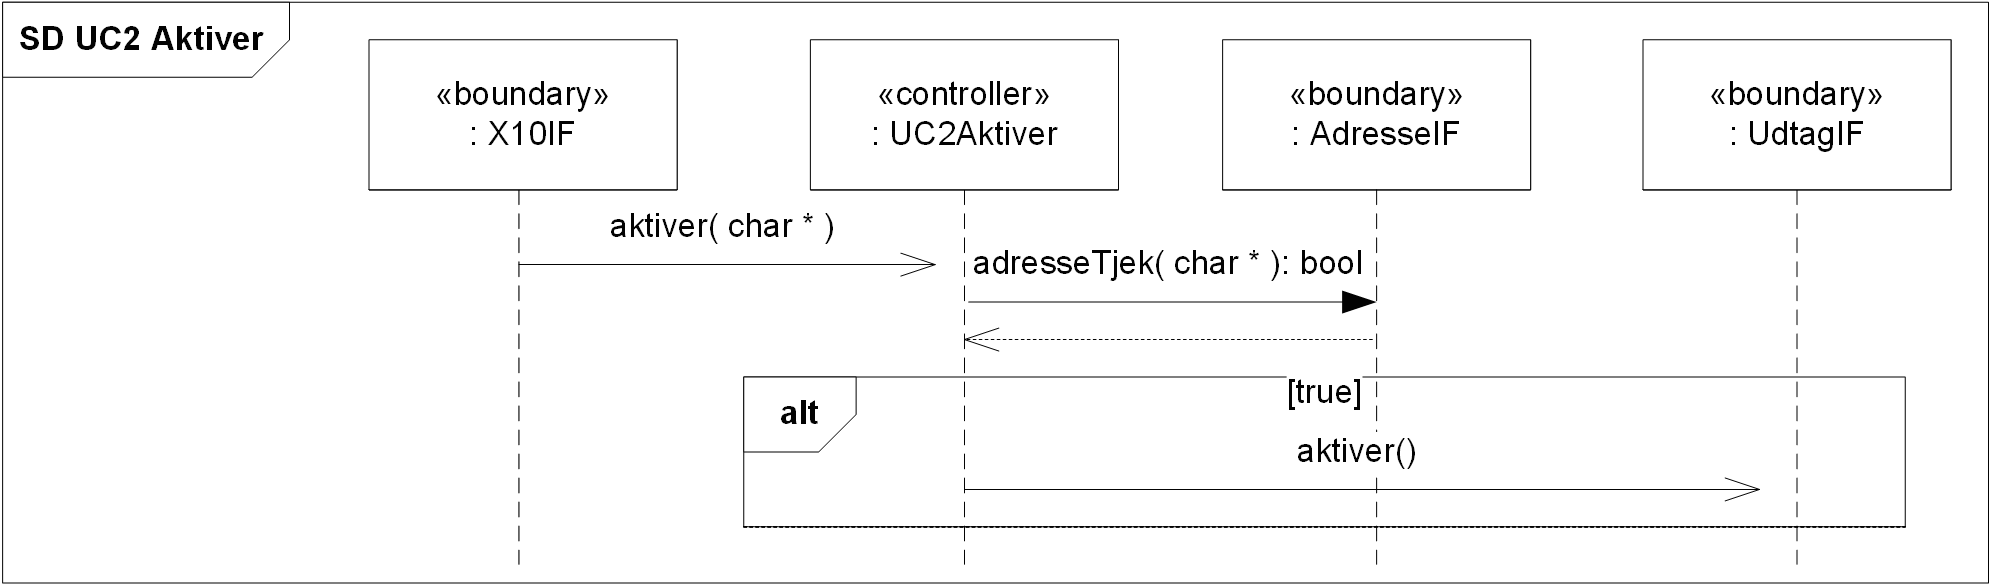
\includegraphics[width=0.9\textwidth]{Billeder/UML/X10_modtager_SD}}
     \caption{Sekvensdiagram for X10 udtag}
     \label{fig:X10_udtag_sd}
\end{figure}

Dette resulterer i et klassediagram med grundfunktionaliteten beskrevet, se figure \ref{fig:X10_udtag_class}. Denne bruges under implementeringen og ender ud i et statisk klassediagram som beskriver det endelige program med alle hjælpemetoder.

\begin{figure}[!htb]
     \centering
     { 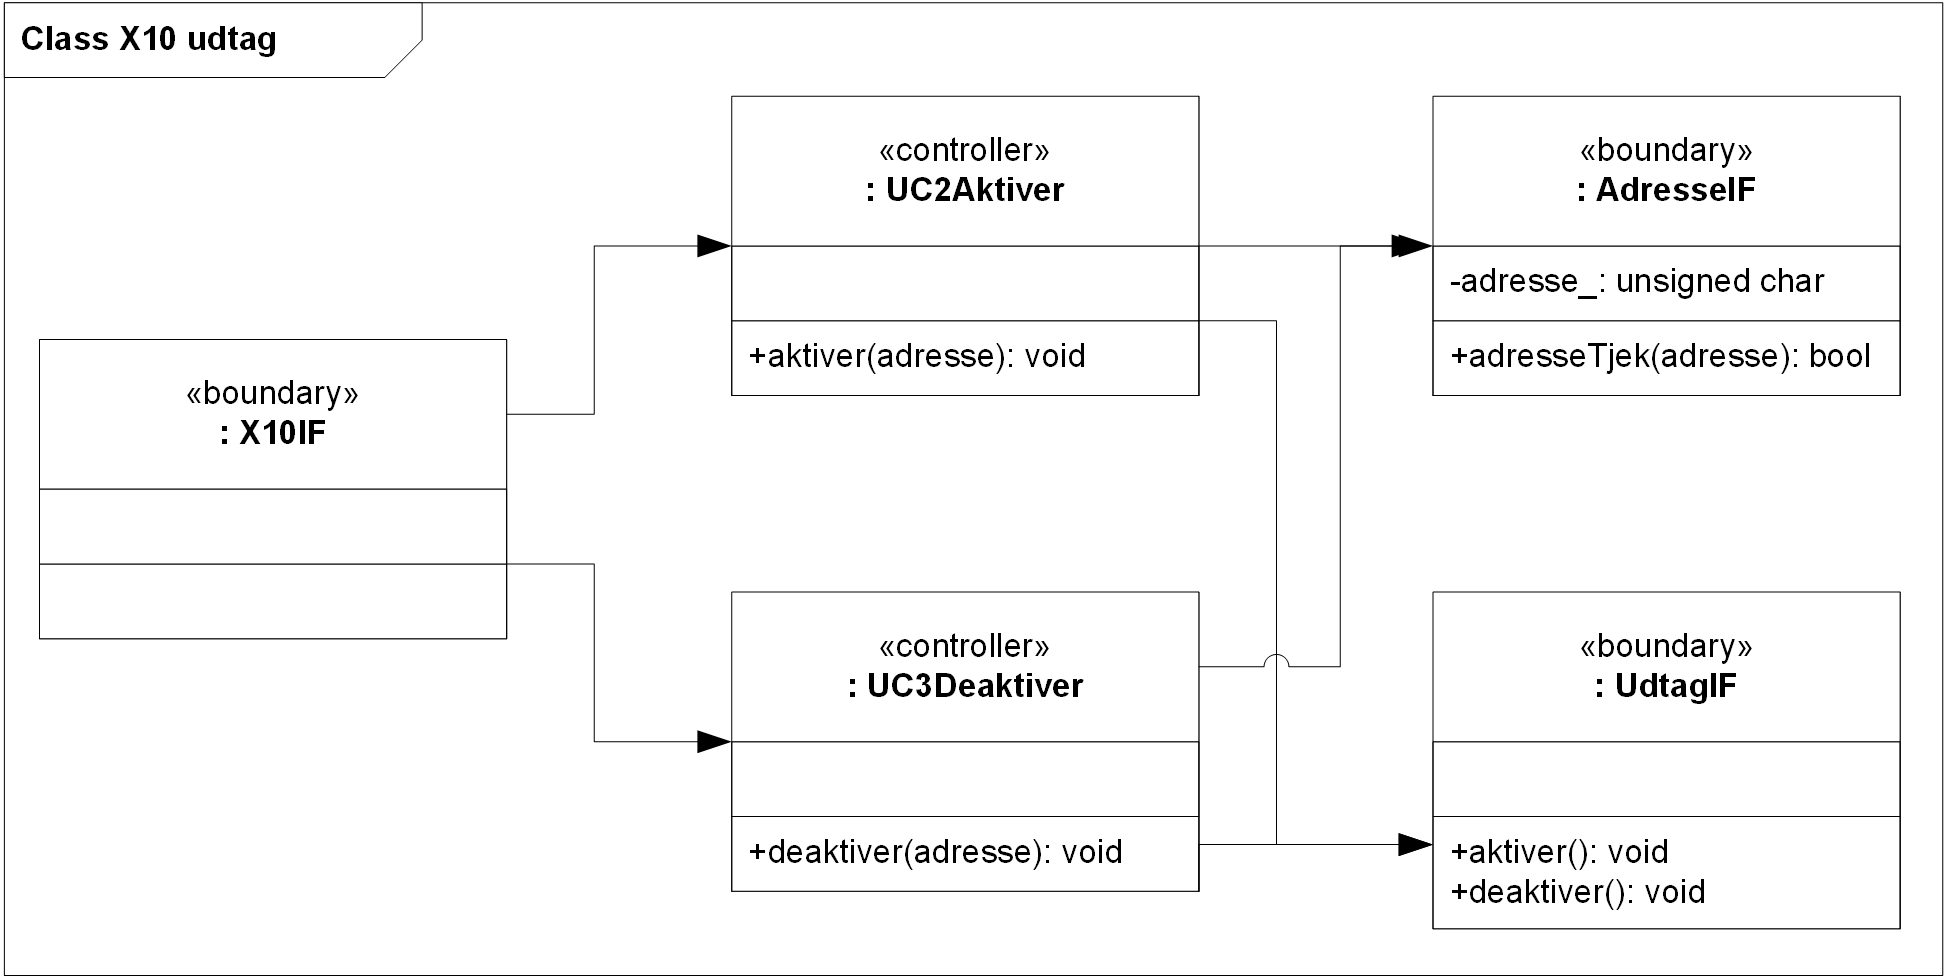
\includegraphics[width=0.9\textwidth]{Billeder/UML/X10_modtager_Class}}
     \caption{Klassediagram for X10 udtag}
     \label{fig:X10_udtag_class}
\end{figure}

Denne analyse af funktionalitet giver et klart overblik til implementeringsfasen.